\subsection{Backend}

O desenvolvimento do \textit{backend} constituiu uma das partes fundamentais do projeto, assegurando a implementação da lógica de negócio, a gestão dos dados e a comunicação entre o sistema e a interface de utilizador. Este componente atua como a camada central responsável por garantir que os processos internos sejam executados de forma consistente, segura e eficiente, proporcionando suporte às funcionalidades disponibilizadas no \textit{frontend}.  

Nesta secção irá se apresentar funcionalidades do backend no contexto da US3 (definida na tabela \ref{tab:req-funcionais}).







\subsubsection{Spring}
\label{sec:backend-Spring}

A framework Spring apresentou à equipa uma alta curva de aprendizagem. Os vários conceitos e ferramentas nesta são bastante alienígenas a qualquer outra ferramenta antes utilizada pelos membros. Por tal foi necessário mais tempo para a aprender. Alguns dos conceitos-chave considerados incluem:

\begin{itemize}
    \item \textbf{\textit{Spring Data}} é um agregado de módulos Spring que têm como função principal facilitar a programção de entidades e o seu respetivos acesso quando conectado a uma fonte de dados.

    \item \textbf{\textit{Spring Data JPA}} (ou só \textit{JPA}) é um dos módulos pertencente à coletânea Spring Data. O seu objetivo é facilitar a implementação de repositórios, reduzindo estes a interfaces Java, nas quais o Spring analisa o nome do método e implementa em \textit{runtime} o mesmo. 

    \item \textbf{\gls{Hibernate}} \cite{docs-hibernate} é uma framework Java e uma solução \GLSxtrshort{ORM} que serve como implementação do \textit{JPA} para, logicamente, persistir a informação na respetiva base de dados.

    \item \textbf{\GLSxtrshort{IoC}} (\acrlong{IoC}, em português \textit{Inversão de Controlo}) é um princípio de engenharia de \textit{software} que transfere a responsabilidade pela criação e gestão dos objetos para uma \textit{framework} específica. No \textit{Spring}, esta funcionalidade é desempenhada pelo denominado \textit{\GLSxtrshort{IoC} Container}.
    
    \item \textbf{\textit{Bean}} corresponde a uma instância de objeto gerida pelo \textit{\GLSxtrshort{IoC} Container}. Cada \textit{Bean} é criado, configurado e mantido pelo próprio contentor, segundo a configuração definida.
    
    \item \textbf{\GLSxtrshort{DI}} (\acrlong{DI}, em português \textit{Injecção de Dependências}) é um princípio amplamente utilizado no desenvolvimento de \textit{software} que visa reduzir o acoplamento entre classes. No contexto do \textit{Spring}, esta prática é suportada através do \textit{IoC Container}, que fornece e gere as instâncias necessárias sob a forma de \textit{Beans}.
    
\end{itemize}









\subsubsection{Estrutura de pastas}

A estrutura de pastas do backend foi definida para enaltecer a função de cada ficheiro e/ou classe em cada uma, como pode ser observado na figura \ref{fig:folder-struct-backend}.

\begin{figure}[h!tbp]
    \centering
    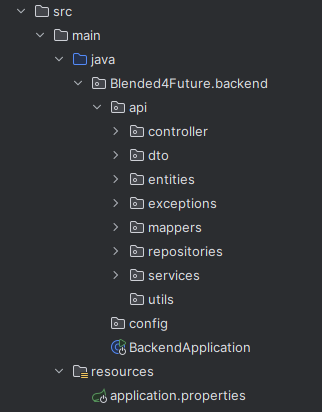
\includegraphics[width=0.5\linewidth]{capitulos/cap4-implementacao/assets/fold-struct-backend.png}
    \caption{Estrutura de pastas do backend}
    \label{fig:folder-struct-backend}
\end{figure}

\subsubsection{Entidades e relações}

Para o caso de uso a ser considerado, a entidade de maior importância será \textit{Project}. Esta encontra-se representada na figura \ref{lst:classe-projeto}.

Em nota, interessante enaltecer o uso das respetivas anotações:

\begin{itemize}
    \item \textbf{\textit{@Entity}} informa o \GLSxtrshort{JPA}/\gls{Hibernate} que esta é uma entidade que deve ser persistida. Para tal deve conter um argumento anotado \lstinline|@Id|.
    \item \textbf{\textit{@Data}}\cite{docs-annotation-data} serve como substituto para as anotações \lstinline|@ToString|, \lstinline|@EqualsAndHashCode|, \lstinline|@Getter|, \lstinline|@Setter| e \lstinline|@RequiredArgsConstructor| que, respetivamente: 
    
    \begin{itemize}
        \item implementa o método \lstinline|toString()| incluindo todos os parâmetros não estáticos da classe;
        \item implementa o método \lstinline|equals(Object object)| e \lstinline|hashCodeO()|. Uma definição (\lstinline|callSuper|) teve de ser subscrita, pois era desejado inclusão dos atributos da superclasse \lstinline|BaseEntity| neste método (ver secção \ref{sec:base-entity});
        \item implementa métodos \textit{getter} para todos os atributos privados
        \item implementa metodos \textit{setter} para todos os atributos privados
        \item implementa um construtor com um parâmetro por atributo não final da classe.
    \end{itemize}

\end{itemize}

\begin{lstlisting}[language=Java, caption={Classe \textit{Project}}, label={lst:class-project}]
@Entity
@Data
@EqualsAndHashCode(callSuper = true)
public class Project extends BaseEntity {

    @Column(nullable = false)
    @Convert(converter = ProjectName.NameConverter.class)
    private ProjectName name = new ProjectName();

    @Column(nullable = false)
    @Convert(converter = ProjectDescription.DescriptionConverter.class)
    private ProjectDescription description = new ProjectDescription();

    @ManyToOne
    private Company company;

    @ManyToOne
    private CompanyRepresentative companyRepresentative;

    @ManyToMany
    private Set<Student> students = Set.of();

    @ManyToMany
    private Set<Qualification> qualifications = Set.of();

    @OneToMany(mappedBy = "project", cascade = CascadeType.REMOVE)
    private Set<Report> reports = Set.of();

    @ManyToOne
    private CourseEdition courseEdition;
}
\end{lstlisting}













\subsubsection{\textit{BaseEntity}}
\label{sec:backend-base-entity}

Como medida de segurança e de padronização, foi desenvolvida a classe \textit{BaseEntity} (ver listagem \ref{lst:backend-base-entity}). Esta classe define dois identificadores: um interno e um externo. O identificador externo é utilizado na comunicação com o cliente, sendo retornado nos pedidos sob a forma de \textit{DTO}, enquanto o identificador interno é reservado para uso exclusivo do sistema.

Tal como o próprio nome indica, a \textit{BaseEntity} foi concebida para servir como \textit{superclasse} de todas as entidades persistentes.

A implementação da \textit{BaseEntity} envolve várias decisões de \textit{design} que merecem atenção:

\begin{itemize}
    \item No \gls{Hibernate}, os atributos definidos em superclasses não são, por defeito, persistidos. A utilização da anotação \lstinline|@MappedSuperclass| assegura que as classes filhas possam herdar esses parâmetros, permitindo a sua correta persistência na base de dados.

    \item A anotação \lstinline|@Id| define o atributo \lstinline|iid| como identificador principal da entidade no contexto da persistência. Complementarmente, \lstinline|@GeneratedValue(strategy=GenerationType.UUID)| especifica a forma como o identificador deve ser gerado, recorrendo ao padrão \textit{UUID}. Esta opção é particularmente relevante dado que, por omissão, o \gls{Hibernate} apenas consegue popular atributos de tipos primitivos.
    
    \item Verificou-se a necessidade de avaliar, de forma global, todos os atributos relacionados com a lógica de negócio, de modo a identificar e retornar eventuais erros existentes. Para esse fim, a função \lstinline|isBusinessDataValid()| analisa todos os \textit{Value Objects} (Ver secção \ref{sec:backend-value-objects}) da respetiva classe e devolve um \lstinline|HashMap| contendo a listagem dos erros detetados.
\end{itemize}

\begin{lstlisting}[language=Java,caption={Classe \textit{BaseEntity}},label={lst:base-entity}]
@MappedSuperclass
@Getter
public abstract class BaseEntity {

    @Id
    @GeneratedValue(strategy = GenerationType.UUID)
    private UUID iid;

    @Column(name="eid", unique = true, nullable = false)
    private UUID externalId;

    public BaseEntity() {
        this.externalId = generateCode();
    }

    private UUID generateCode() {
        return UUID.randomUUID();
    }

    public HashMap<String, Object> isBusinessDataValid() {

        HashMap<String, Object> errors = new HashMap<>();

        Class<?> clazz = this.getClass();
        List<IValueObject<?>> valueObjects = new ArrayList<>();

        while (clazz != null && clazz != Object.class) {
            for (Field field : clazz.getDeclaredFields()) {
                field.setAccessible(true);
                try {
                    Object value = field.get(this);

                    if (value instanceof IValueObject<?> vo) {
                        valueObjects.add(vo);
                    }
                } catch (IllegalAccessException ignored) {}
            }
            clazz = clazz.getSuperclass();
        }

        return isBusinessDataValid(valueObjects);
    }

    public static HashMap<String, Object> isBusinessDataValid(List<IValueObject<?>> fields) {
        HashMap<String, Object> errors = new HashMap<>();
        for (IValueObject<?> field : fields) {
            if (field == null) {
                continue;
            }
            errors.putAll(field.isValid());
        }
        return errors;
    }
}

\end{lstlisting}












\subsubsection{\textit{Value Objects}}
\label{sec:backend-value-objects}

A utilização de \textit{Value Objects} permite um maior controlo sobre a lógica de negócio inerente ao projeto. Por tal a sua implementação é necessária aquando a construção de um sistema de superior complexidade. 

A listagem \ref{lst:interface-value-object} mostra a interface \lstinline|ValueObject|.

\begin{lstlisting}[language=Java,caption={Interface \textit{Value Object}},label={lst:interface-value-object}]
public interface IValueObject<T> {
    T getValue();
    public HashMap<String, Object> isValid();
}
\end{lstlisting}

A notar, a função \lstinline|isValid()| em conjunto com a superclasse \lstinline|BaseEntity| permite verificar a lógica de negócio de cada respetivo \lstinline|ValueObject|. Para tal basta implementação fazer uma verificação do objecto em questão e retornar um \lstinline|HashMap| com toda a informação de erros.

\begin{lstlisting}[language=Java,caption={Classe \textit{ProjectDescription}},label={lst:class-project-description}]
@Value
public class ProjectDescription implements IValueObject<String> {

    public static final int MIN_LENGTH = 10;
    public static final int MAX_LENGTH = 500;
    public static final String DEFAULT_DESCRIPTION = "Default Project Description";

    private String description;

    @Override
    public String getValue() {
        return this.description;
    }

    public ProjectDescription(String value) {
        this.description = value;
    }

    public ProjectDescription() {
        this(DEFAULT_DESCRIPTION);
    }

    @Override
    public HashMap<String, Object> isValid() {
        HashMap<String, Object> errors = new HashMap<>();
        if (this.getValue() == null || this.getValue().isEmpty()) {
            errors.put("description", "Description cannot be null or empty");
        } else if (this.getValue().length() < MIN_LENGTH || this.getValue().length() > MAX_LENGTH) {
            errors.put("description", "Description must be between 10 and 500 characters long");
        }
        return errors;
    }

    @Converter
    public static class DescriptionConverter implements jakarta.persistence.AttributeConverter<ProjectDescription, String> {
        @Override
        public String convertToDatabaseColumn(ProjectDescription description) {
            return description.getValue();
        }

        @Override
        public ProjectDescription convertToEntityAttribute(String dbData) {
            return new ProjectDescription(dbData);
        }
    }
}
\end{lstlisting}

A listagem \ref{lst:class-project-description} demonstra uma implementação de \lstinline|IValueObject|. Como referido a função \lstinline|isValid()| avalia se o objeto é valido ou não retornando quaisquer erros.

Importante também seria referir a necessidade de um conversor, uma classe que informa o \gls{Hibernate} como deve mapear o objeto do programa para a base de dados e vice-versa.







\subsubsection{Repositórios}

Como referido na secção \ref{sec:backend-Spring}, o modulo Spring Data \GLSxtrshort{JPA}, permite a implementação de repositórios em \textit{runtime}.

Tendo em conta a implementação de \lstinline|BaseEntity| e a necessidade de diferenciação entre identificadores internos e externos, foi implementada a interface \lstinline|BaseRepository| (ver listagem \ref{lst:interface-base-repository}). 

Na referida interface o uso de \lstinline|@NoRepositoryBean| informa o \GLSxtrshort{IoC} \textit{Container} para não guardar uma instância deste repositório, pois por norma todos os \lstinline|JpaRepository| são guardados automaticamente. É ainda adicionada a função \lstinline|findByExternalId|, esta procura automaticamente por todas a instâncias que o correspondem ao nome do atributo \lstinline|externalId|. Esta segue uma nomenclatura especifica do Spring \cite{docs-spring-repository}.

\begin{lstlisting}[language=Java,caption={Inteface BaseRepository}, label={lst:interface-base-repository}]
@NoRepositoryBean
public interface BaseRepository<T extends BaseEntity> extends JpaRepository<T, UUID> {
    Optional<T> findByExternalId(UUID internalId);
}
\end{lstlisting}

Graças ao \gls{Spring} é possível então fazer implementações de repositórios muito facilmente, como exemplificado na listagem \ref{lst:interface-project-repository}

\begin{lstlisting}[language=Java, caption={interface \textit{ProjectRepository}}, label={lst:interface-project-repository}]
    public interface ProjectRepository extends BaseRepository<Project> {}
\end{lstlisting}







\subsubsection{Controladores e prevenção de erros}

Na eventualidade da ocorrência de erros, que estes sejam de negócio ou de sistema torna-se necessária implementar um sistema que os consiga detetar e retornar num formata predefinido, algo que o \gls{Spring} não faz por base. 

O \gls{Spring} disponibiliza \lstinline|@RestControllerAdvice| que permite a implementação de rotas ou ferramentas de deteção de erros em todas as classes anotadas com \lstinline|@RestController|.

Na listagem \ref{lst:class-AppExceptionController} entende-se o elemento base que permite capturar erros internos ou de negócio e retorná-los num formato predefinido (ver listagem \ref{lst:class-Error}). Em prática a anotação \lstinline|@ExceptionHandler(AppException.class)| faz com que a qualquer ponto de execução do programa, no caso de ser lançada uma exceção do tipo \lstinline|AppException| a esta se redirecione para a função \lstinline|handleAppException|. Na listagem \ref{lst:class-ProjectController} e \ref{lst:exception-AppException} mostra-se, respetivamente, exemplo do uso desta exceções e propria exceção \lstinline|AppException|.

\begin{lstlisting}[language=Java, caption={Class \textit{AppExceptionController}}, label={lst:class-AppExceptionController}]
@Slf4j
@RestControllerAdvice
@RequiredArgsConstructor
public class AppExceptionController {

    // Everytime an app exception is thrown, this method will be called
    // It will log the error and return a ResponseEntity with the error details
    @ResponseBody
    @ExceptionHandler(AppException.class)
    public ResponseEntity<?> handleAppException(AppException e, HttpServletRequest request) {
        log.error("App Exception occurred: {}", e.getMessage(), e);
        return createResponseError(e, request.getRequestURI());
    }

    private ResponseEntity<ErrorResponse> createResponseError(AppException e, String path) {
        Error err = new Error(
                e.getMessage(),
                e.getStatus().value(),
                path,
                Instant.now(),
                e.getData()
        );

        ErrorResponse errorResponse = ErrorResponse.fromError(err);

        return new ResponseEntity<>(errorResponse,new HttpHeaders(), e.getStatus());
    }

}
\end{lstlisting}

\begin{lstlisting}[language=Java, caption={Class \textit{Error}}, label={lst:class-Error}]
@Value
@AllArgsConstructor(access = PUBLIC)
public class Error {
    String message;
    int status;
    String path;
    Instant timestamp;
    Map<String, Object> data;
}
\end{lstlisting}

\begin{lstlisting}[language=Java, caption={Class \textit{ProjectController}}, label={lst:class-ProjectController}]
@RestController
@RequestMapping("/api/project")
public class ProjectController {


    private final IProjectService service;

    public ProjectController(IProjectService IProjectService) {
        this.service = IProjectService;
    }

    @GetMapping("")
    public List<ProjectDTO> getAllProjects() {
        return service.getProjects();
    }

    @GetMapping("/{id}")
    public ProjectDTO getProjectById(UUID id) {
        try {
            return service.getProject(id);
        } catch (NoSuchElementException e) {
            throw new AppException(e, HttpStatus.NOT_FOUND);
        }
    }

    @PostMapping("")
    public ProjectDTO addProject(@RequestBody AddProjectDTO project) {
        try {
            return service.addProject(project);
        } catch (NoSuchElementException e) {
            throw new AppException(e, HttpStatus.NOT_FOUND);
        } catch (FormDataException e) {
            throw new AppException(e, HttpStatus.BAD_REQUEST, e.getErrors());
        }
    }

    @PutMapping("/{id}")
    public ProjectDTO updateProject(@PathVariable UUID id, @RequestBody @Valid AddProjectDTO project) {
        try {
            return service.updateProject(id, project);
        } catch (NoSuchElementException e) {
            throw new AppException(e, HttpStatus.NOT_FOUND);
        } catch (FormDataException e) {
            throw new AppException(e, HttpStatus.BAD_REQUEST, e.getErrors());
        }
    }

    @DeleteMapping("/{id}")
    public ProjectDTO deleteProject(@PathVariable UUID id) {
        try {
            return service.deleteProject(id);
        } catch (NoSuchElementException e) {
            throw new AppException(e, HttpStatus.NOT_FOUND);
        }
    }
}
\end{lstlisting}

\begin{lstlisting}[language=Java, caption={Exceção \textit{AppException}}, label={AppException}]
@Getter
public class AppException extends RuntimeException{

    private final HttpStatus status;
    private Map<String, Object> data;

    public AppException(String message, HttpStatus status, Map<String, Object> data) {
        super(message);
        this.status = status;
        this.data = data;
    }

    public AppException(Exception e, HttpStatus status, Map<String, Object> data) {
        super(e.getMessage());
        this.status = status;
        this.data = data;
    }

    public AppException(Exception e, HttpStatus status) {
        super(e.getMessage());
        this.status = status;
        this.data = new HashMap<>();
    }

    public AppException(String message, HttpStatus status) {
        super(message);
        this.status = status;
        this.data = new HashMap<>();
    }
}
\end{lstlisting}







\subsubsection{Serviços}

O padrão de \textit{software} \textit{Service} entende a concentração da de toda a lógica de negócio numa só camada do sistema. A listagem \ref{lst:method-create-new-project-class-ProjectService} apresenta a implementação do método \lstinline|addProject| nesta mesma camada.

A notação \lstinline|@Service| permite ao \GLSxtrshort{IoC} \textit{container} identificar esta classe como serviço e guardá-la como \textit{Bean}. Já a notação \lstinline|@Slf4j| cria uma ferramenta utilizada para manter registo de qualquer ação no programa. 

\begin{lstlisting}[language=Java, caption={Implementação do metodo para criação de um novo projeto}, label={lst:method-create-new-project-class-ProjectService}]
@Service
@Slf4j
public class ProjectService implements IProjectService{
    |\Suppressnumber|
    ... 
    |\Reactivatenumber|
    @Override
    public ProjectDTO addProject(AddProjectDTO project) throws FormDataException {

        HashMap<String,Object> errors = checkIdAttributeAddDTO(project);

        ProjectName name = new ProjectName(project.name());
        ProjectDescription description = new ProjectDescription(project.description());

        errors.putAll(
            Project.isBusinessDataValid(
                    new ArrayList<>(List.of(name, description))
            )
        );
        if (!errors.isEmpty()) {
            throw new FormDataException("Project data is not valid", errors);
        }

        Company company = project.companyId() == null ? 
            companyRepository.findByExternalId(project.companyId()).get() : null;

        CompanyRepresentative companyRepresentative =
            project.companyRepresentativeId()==null ? 
            companyRepresentativeRepository.findByExternalId(
                project.companyRepresentativeId()
            ).get() : null;
        
        List<Student> students = project.studentIds() == null ? 
                List.of() : 
                project.studentIds().stream()
                .map(studentRepository::findByExternalId)
                .filter(Optional::isPresent)
                .map(Optional::get)
                .toList();

        CourseEdition courseEdition = 
            project.courseEditionId() == null ? 
            courseEditionRepository.findByExternalId(
                project.courseEditionId()
            ).get() : null;

        Project newProject = new Project();

        newProject.setName(name);
        newProject.setDescription(description);
        newProject.setCompany(company);
        newProject.setCompanyRepresentative(companyRepresentative);
        newProject.setStudents(new HashSet<>(students));
        newProject.setCourseEdition(courseEdition);

        Project savedProject = projectRepository.save(newProject);
        log.info(
            "Project with eid {} created successfully", 
            savedProject.getExternalId()
        );
        return new ProjectMapper().toDTO(savedProject);
    }
    |\Suppressnumber|
    ...
    |\Reactivatenumber|
}

\end{lstlisting}


\subsubsection{Documentação}

De forma a assegurar que os atuais e potenciais futuros desenvolvedores pudessem acompanhar e compreender o trabalho previamente realizado, optou-se pela integração do \textit{Swagger}. Esta ferramenta permite a geração automática de documentação da API, disponibilizando-a por uma interface \textit{Web} centralizada. Para além de facilitar a consulta das funcionalidades já implementadas, o \textit{Swagger} contribui para a padronização da comunicação entre a equipa de desenvolvimento e outros intervenientes, garantindo maior clareza, acessibilidade e manutenção contínua da solução.

\begin{figure}[h!tbp]
    \centering
    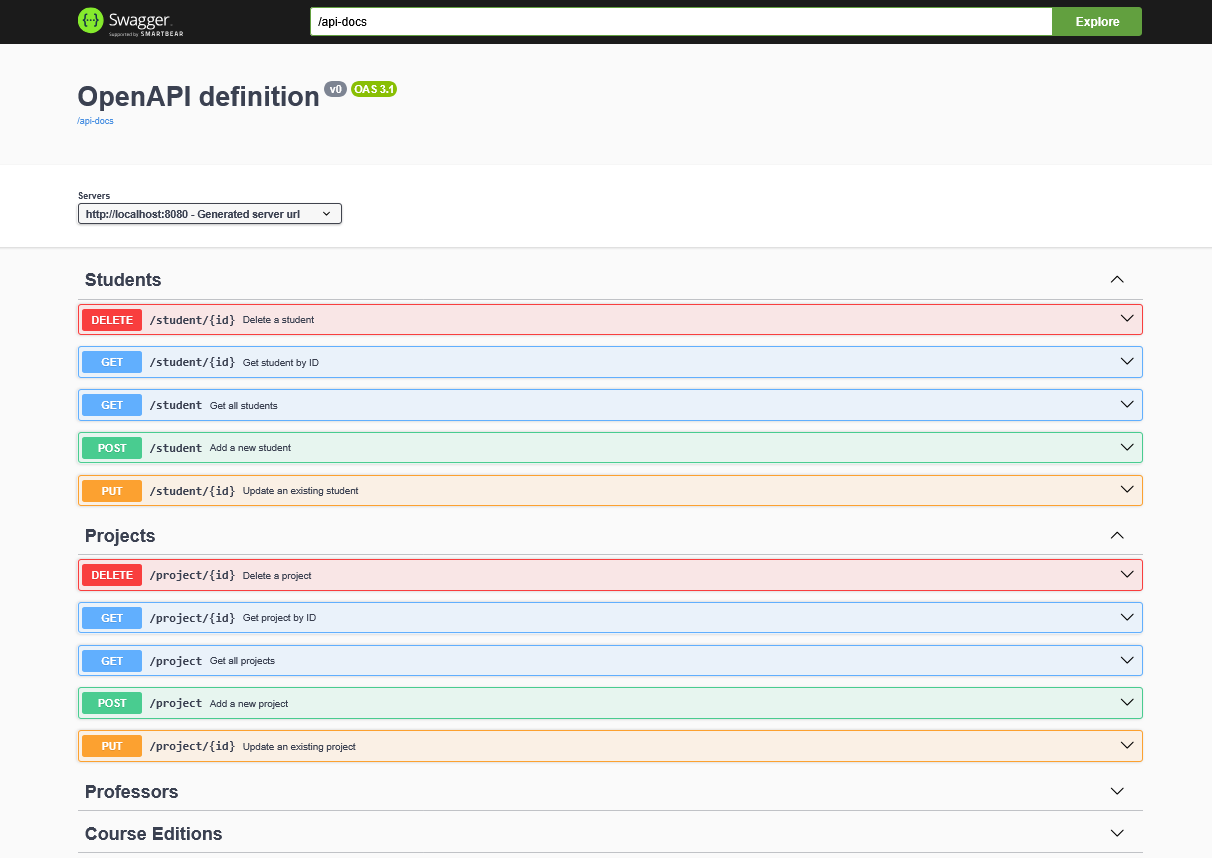
\includegraphics[width=\linewidth]{capitulos/cap4-implementacao/assets/swagger-homepage.png}
    \caption{\textit{Webpage} do \textit{Swagger}}
\end{figure}